\section{Data Description}

We have selected the daily spot price of Brent crude oil and the daily Gas Supply Hub (GSH) \cite{mitch1} trade price of LNG as measures of the price of oil and natural gas in Australia. Brent crude in this context refers to both the dated price of a basket of North Sea crude oils and the contract price of Brent crude oil futures \cite{mitch2}. Whilst the price of South-East Asian crudes such as Malaysian Tapis became a benchmark for Asia-Pacific oil markets in the 1990s, decreasing regional production in past decade have resulted in the establishment of Brent crude as Australia’s benchmark price \cite{mitch3}. 
\medskip

GSH trade price refers to an average of wholesale LNG trade prices across the two AEMO operated gas supply hubs in Wallumbilla, Queensland and Moomba, South Australia \cite{mitch1}. These wholesale trade prices largely function as a benchmark for LNG price across east coast Australia and capture factors such as domestic demand and netback price, the equivalent export value price of LNG \cite{mitch4}.
\medskip

As this report is primarily interested with sanction-driven price patterns, the 21 February 2022, the introduction of sanctions specifically in response to what has become the invasion of Ukraine, has been selected as the point of divergence. Daily data for the two years up to 21 February has been selected to construct the model. Furthermore, 2022 data is available up to 16 May in the case of both oil and LNG. The Brent crude oil dataset is fairly clean yet still contains some missing values. Due to the daily frequency and number of years available it is judged that there is sufficient data to drop these missing values. The monthly LNG hub price dataset is comparatively messy with isolated price spikes and additional price forecasts. These isolated spikes are an undesirable result of using monthly data, however, a lack of transparency within the Australian gas market, results in difficulty finding higher frequency data. To counteract this, it was decided more years of LNG data were to be included in the modelling to compensate. The dataset is otherwise complete, and the forecast data can be dropped.

% Brent Crud price over time

\begin{figure}[H]
    \centering
    \subfloat[\centering Brent Crude price]{{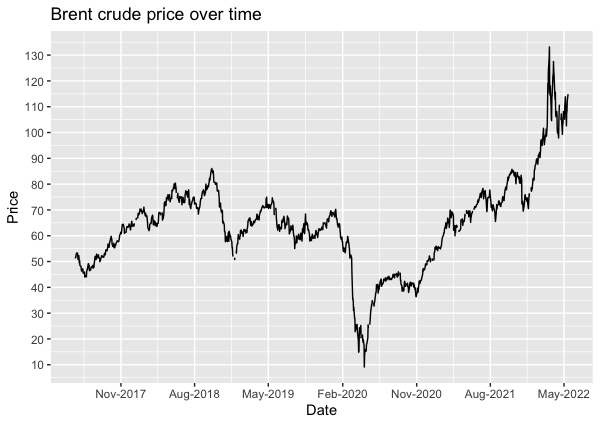
\includegraphics[width=7cm]{Figures/Data-desc/Brent-crude-price.png} }}%
    \caption{Brent Crude price between late 2017 and mid 2022}%
    \label{fig:Brent-Crude-price}%
\end{figure}

\subsection{Time Series Visualisation}

Visual analysis of our Brent crude data reveals a steady two year trend before a clear period of increased price volatility beginning on 25 February 2022. This is most evident over March there are two large price spikes and subsequent drops. The largest of these saw price increasing from \$103.08 USD per barrel to over \$133 USD in eight days. This spike coincides with the exclusion of select Russian banks from the SWIFT system on the 26th \cite{mitch5}, and the sale of BP’s 19.75\% stake in state-controlled oil company Rosneft on the 27th \cite{mitch6}. Notably, there is a four day delay between the initial introduction of tariffs and this price jump, suggesting the Russian invasion on the 24th as a more likely cause. The presence of these spikes late in our dataset also suggest heteroskedasticity as a potential issue. By selecting 21 February as the cutoff date for our counterfactual forecast data we do not include this late period of volatility, thus avoiding this late onset heteroskedasticity.

\begin{figure}[H]
    \centering
    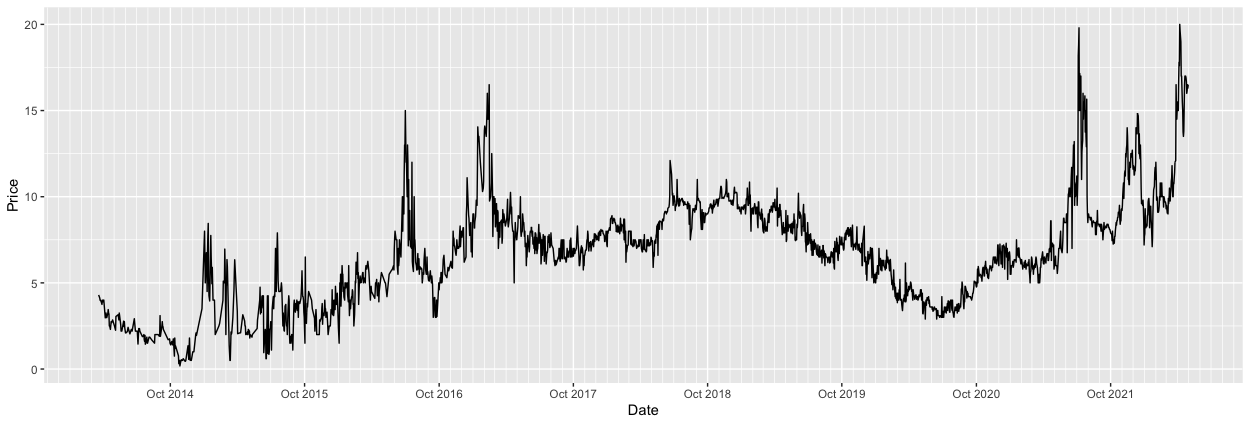
\includegraphics[width=.8\textwidth]{Figures/Data-desc/GSH trade price.png}
    \caption{Results bar graph}
    \label{fig:GSH-trade-price}
\end{figure}

By comparison, our LNG dataset does not appear to show a clear pattern of post invasion pricing. Historical GSH data shows a price fall from around \$12/GJ in late February 2022 to \$9/GJ in early March, followed by a spike of \$10/GJ until early April. Despite this, there is evidence of similar price rises and falls occurring even before the introduction of sanctions and the invasion of Ukraine. From October to December 2021 wholesale Australian prices approximately doubled, largely in response to upward demand for LNG from Asia in expectation of a colder Northern Hemisphere Winter \cite{mitch7}. The instance of sudden December price rises occurring in 2014, 2016 and 2021 could indicate some seasonality but the lack of a consistent yearly pattern is counter-intuitive. Visual analysis of seasonality in our LNG price data is thus inconclusive. As before, volatility increases throughout 2022, the end of our dataset, suggesting that heteroskedasticity remains a concern. This is also partially avoided by removing post-sanction data when constructing our forecast.

\subsection{Augmented Dickey Fuller Test}

\begin{table}[H]
\centering
% \setlength{\tabcolsep}{5pt} % Default value: 6pt
% \renewcommand{\arraystretch}{1.5} % Default value: 1
\caption{Augmented Dickey-Fuller Test Results}
\begin{tabular}{c|cc}
            & No Trend & Trend\\\hline\hline
Brent Crude & -1.7373 & -2.5021\\\hline
Henry Hub & -2.5264 & -4.3439**
\end{tabular}\label{Tab:ADF_LNG}
\\
* Significant at the 5\% level\\
** Significant at the 1\% level
\end{table}

We test both datasets for autocorrelation using an augmented Dickey-Fuller (ADF) test with and without trend. Akaike information criteria suggests selecting lags equal to one. Results from the ADF test suggests there is only statistically significant evidence of trend stationarity in our LNG supply hub price data.

\subsection{ADF and PACF Visual Analysis}

\begin{figure}[H]
    \centering
    \subfloat[\centering LNG netback ACF]{{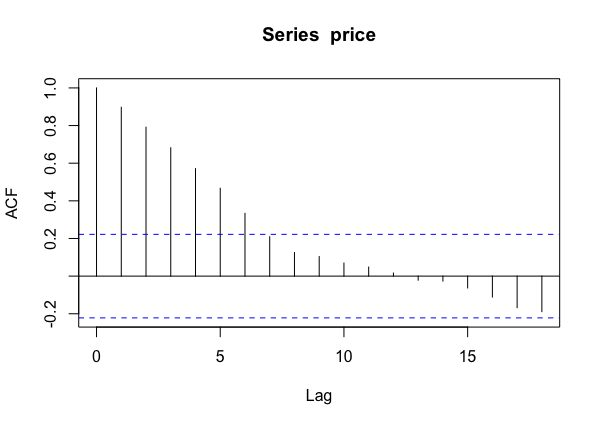
\includegraphics[width=0.4\textwidth]{Figures/Data-desc/LNG netback ACF.png} }}%
    \qquad
    \subfloat[\centering LNG netback PACF]{{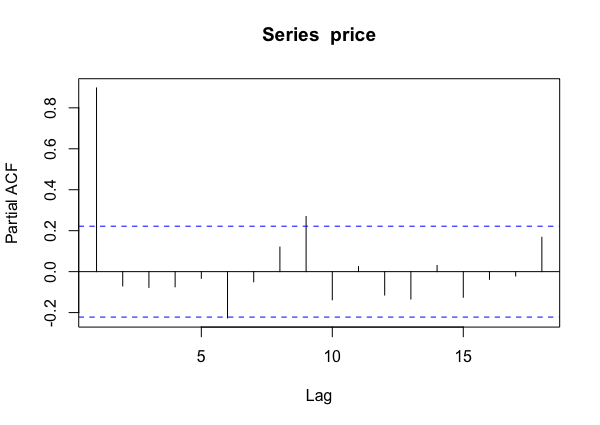
\includegraphics[width=0.4\textwidth]{Figures/Data-desc/LNG netback PACF.png} }}%
    \caption{LNG netback}%
    \label{fig:example3}%
\end{figure}

Analysing our ACF for our Brent crude data reveals a decay to zero, suggesting at least some minimal stationarity despite not finding statistically significant evidence in our ADF test. Furthermore, whilst there are comparatively large lags in our PACF there appears to be no clear seasonal pattern. This would support the conclusion there is little seasonality in crude oil prices.

\begin{figure}[H]
    \centering
    \subfloat[\centering GSH trade price ACF]{{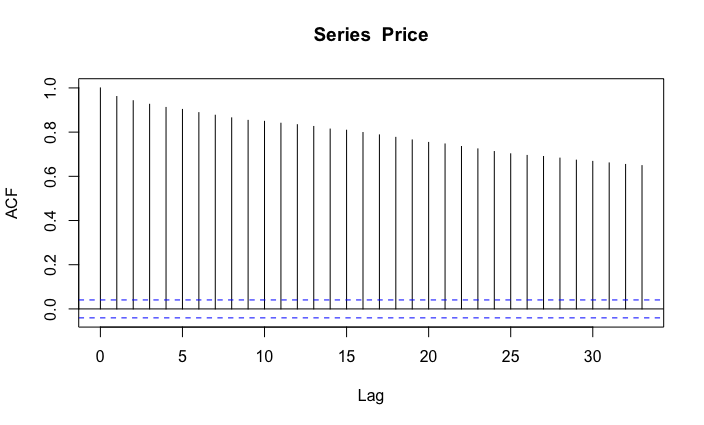
\includegraphics[width=0.4\textwidth]{Figures/Data-desc/GSH trade price ACF.png} }}%
    \qquad
    \subfloat[\centering GSH trade price PACF]{{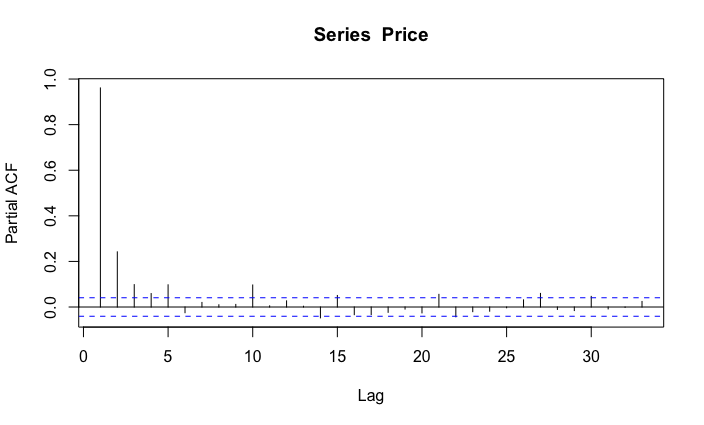
\includegraphics[width=0.4\textwidth]{Figures/Data-desc/GSH trade price PACF.png}{F} }}%
    \caption{GSH trade price}%
    \label{fig:example4}%
\end{figure}

Our LNG supply hub price data shows an even more gradual linear decay in the ACF as would be expected from non-stationary data. This is consistent with the trend-stationarity identified in our ADF test. The PACF graph illustrates a muddied pattern of larger lags decaying occurring at 5, 10, 15, 21, and 27 after an initial decay from 1. This averages out to a season of about 5-6 months. This is reasonable considering the 6 month delay between Southern and Northern hemisphere winters, which could explain these seasonally higher gas prices. Despite this, given a lack of corroborating evidence in our ACF and time series graph suggests this seasonality is likely spurious.
\medskip

Overall, we find both our Brent crude oil and our supply hub LNG trade price data is largely non-stationary. Despite this, ADF test results suggest LNG price may be stationary when de-trended. We find insufficient evidence of seasonality in either dataset.